\documentclass{article}
\usepackage[a4paper, margin=5em]{geometry}
\usepackage{fancyhdr}
\usepackage{lastpage}
\usepackage{graphicx}
\usepackage{hyperref}
\usepackage{ngerman}
\usepackage{enumitem}
\usepackage{csquotes}
\usepackage{caption}

\newcommand{\gqq}[1]{\glqq{}#1\grqq{}}

\pagestyle{fancy}
\fancyhf{}
\renewcommand{\headrulewidth}{0pt}
\fancyfoot{}

\lfoot{}
\cfoot{Seite \thepage\ / \pageref*{LastPage}}
\rfoot{}

\hypersetup{
    colorlinks=true,
    linktoc=all,
    urlcolor=blue
}

\author{Tim Wende}
\date{\today}
\title{\textbf{Hausaufgabe 6}}

\begin{document}
    \maketitle

    \begin{figure}[ht]
        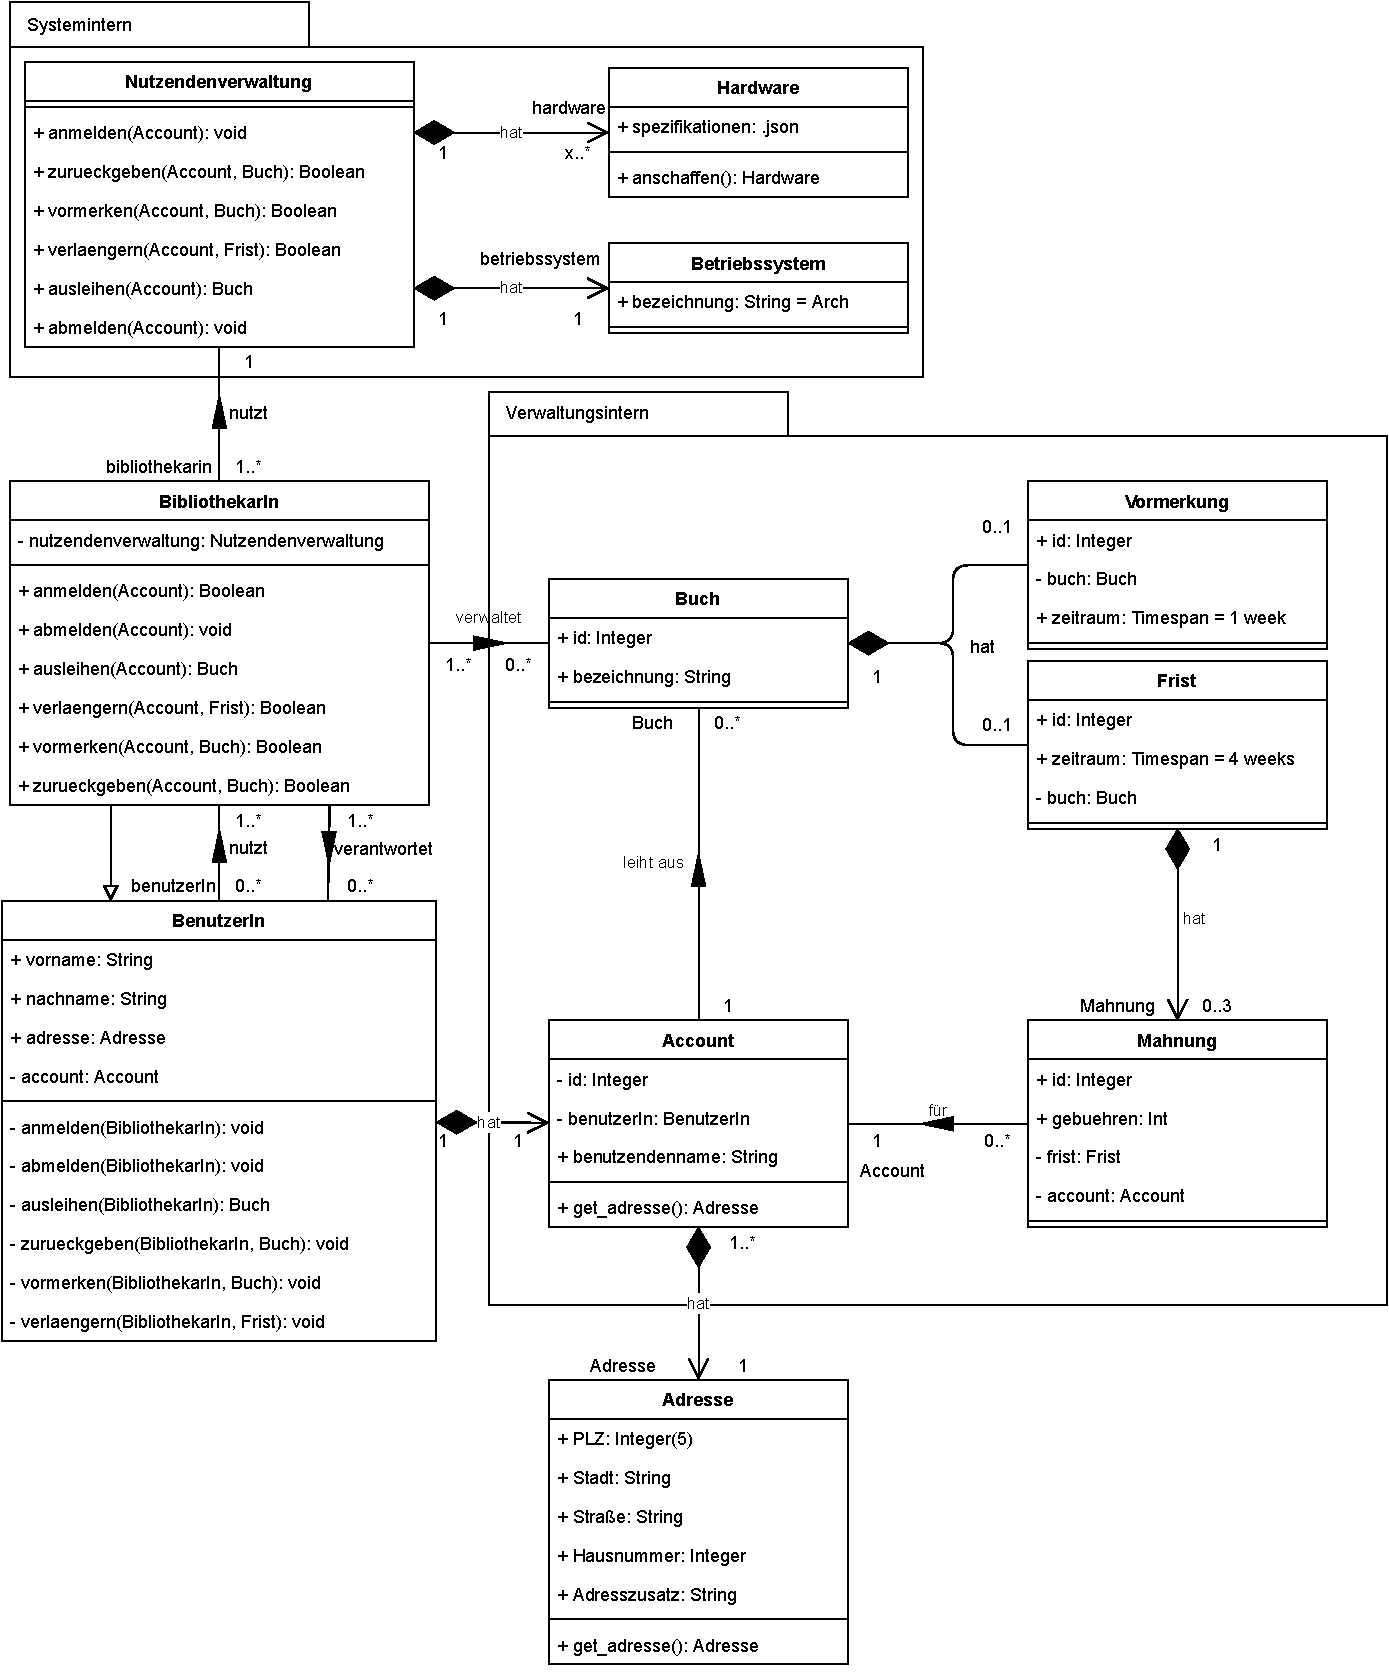
\includegraphics[width=0.9\textwidth]{swt_wende_tim_h06_class_diagram.pdf}
        \caption{\texttt{class\_diagram}}
    \end{figure}

    \newpage
    Liste offener Fragen:
    \begin{itemize}
        \item Ich habe mal unsere allseits bekannten Kompositionspfeile wie bei \href{https://de.wikipedia.org/wiki/Klassendiagramm}{Wikipedia} zu sehen benutzt.
            Da dies nicht in den ursprünglichen UML-Spezifikationen steht, sei dies hier erwähnt.
        \item Die Klasse \texttt{Frist} benötigt noch eine Methode \texttt{mahnung\_versenden()}.
            Da ich diese jedoch über einen externen Event Handler geplant habe, findet sie in diesem Diagramm keinen Platz.
            Dieser sollte automatisch nach Ablauf der Zeitspanne getriggert werden und die Frist im Anschluss erneut erhöhen.
        \item Da die Rollen im Klassendiagramm größtenteils dem Namen der Klasse entspricht, habe diese hauptsächlich als Attribut dargestellt.
            Vor allem außerhalb der Verwaltungsinternen Zone ließ sich das Diagramm so deutlich vereinfachen. 
    \end{itemize}

    \section*{Glossar}
    \textbf{abmelden} schwaches Verb - sich ausloggen; eine Community im Internet [dauerhaft] verlassen \\
    \textbf{Account} Substantiv, Neutrum - Zugangsberechtigung, z. B. zum Internet, einer Datenbank, einem Netzwerk, \ldots\\
    \textbf{Adresse} Substantiv, feminin - Angabe von jemandes Namen und Wohnung, Anschrift\\
    \textbf{Adresszusatz} Substantiv, Neutrum - Zusätzliche Angaben zu der Adresse\\
    \textbf{anmelden} schwaches Verb - bei einer zuständigen Stelle (Behörde, Institution o. Ä.) eintragen lassen\\
    \textbf{anschaffen} schwaches Verb - etwas erwerben, was länger Bestand hat, nicht zum direkten Verbrauch bestimmt ist\\
    \textbf{Arch} Exemplarisches Betriebssystem, welches aus \href{https://www.reddit.com/r/LinuxPorn/}{Gründen} als default Wert genommen wurde. \\
    \textbf{ausleihen} starkes Verb - sich etwas, jemanden bei jemandem leihen\\
    \textbf{BenutzerIn} Substantiv, Neutrum - Person, die etwas [leihweise] benutzt\\
    \textbf{Betriebssystem} Substantiv, Neutrum - System von Programmen für die Steuerung eines digitalen Gerätes\\
    \textbf{Bezeichnung} Substantiv, feminin - Kennzeichnung, Markierung\\
    \textbf{BibliothekarIn} Substantiv, Neutrum - wissenschaftlich ausgebildeter Betreuer, Verwalter einer Bibliothek\\
    \textbf{Boolean} Eine boolesche Variable ist eine Variable, die nur endlich viele Werte oder Zustände annehmen kann.\\
    \textbf{Buch} Substantiv, Neutrum - größeres, gebundenes Druckwerk; Band\\
    \textbf{Frist} Substantiv, feminin - für einen bestimmten Zweck festgelegte Zeitspanne\\
    \textbf{Gebühren} Substantiv, feminin - für eine [öffentliche] Dienstleistung zu bezahlender Betrag\\
    \textbf{Hardware} Substantiv, feminin - Gesamtheit der technisch-physikalischen Teile einer Datenverarbeitungsanlage\\
    \textbf{Hausnummer} Substantiv, feminin - Nummer, mit der die einzelnen Häuser einer Straße bezeichnet sind\\
    \textbf{ID} Substantiv, feminin - Kurzwort für Identifikationsnummer\\
    \textbf{Identifikationsnummer} Substantiv, feminin - Nummer, die eine exakte Zuordnung zu einem Datensatz ermöglicht\\
    \textbf{Integer} Mit Integer wird in der Informatik ein Datentyp bezeichnet, der ganzzahlige Werte speichert\\
    \textbf{Mahnung} Substantiv, feminin - Aufforderung, etwas zu erledigen, Erinnerung an eine Verpflichtung\\
    \textbf{Nachname} Substantiv, maskulin - Familienname [mit vorangestelltem Geburtsnamen]\\
    \textbf{Nutzendenverwaltung} Substantiv, feminin -  Verschiedene Tätigkeiten für die Verwaltung von Benutzenden.\\
    \textbf{PLZ} Abkürzung Post­leit­zahl\\
    \textbf{Post­leit­zahl} Substantiv, feminin - Kennzahl eines Ortes (als Bestandteil der Postanschrift)\\
    \textbf{Spezifikationen} Substantiv, feminin - das Spezifizieren\\
    \textbf{Stadt} Substantiv, feminin - größere, dicht geschlossene Siedlung\\
    \textbf{Straße} Substantiv, feminin - befestigter Verkehrsweg für Fahrzeuge und Fußgänger\\
    \textbf{String} Zeichenfolge variabler Länge\\
    \textbf{Systemintern} Für das System benötigte/ genutzte Zone\\
    \textbf{verlängern} schwaches Verb - länger machen\\
    \textbf{Verwaltungsintern} Für die Verwaltung benötigte/ genutzte Zone\\
    \textbf{Void} Platzhalter für einen leeren Datentypen\\
    \textbf{vormerken} schwaches Verb - jemanden, etwas im Voraus als zu berücksichtigend eintragen\\
    \textbf{Vormerkung} Substantiv, feminin - das Vormerken; das Vorgemerktwerden\\
    \textbf{Vorname} Substantiv, maskulin - Name, der die Individualität einer Person kennzeichnet\\
    \textbf{Zeitraum} Substantiv, maskulin - Verlauf der Geschehnisse erfüllter Teil der Zeit; Zeitabschnitt\\
    \textbf{zurückgeben} starkes Verb - wieder dem [ursprünglichen] Besitzer o. Ä. übergeben\\

    Vielen Dank an den \href{https://www.duden.de/}{Duden} und \href{https://de.wikipedia.org/}{Wikipedia} für das Ausfüllen dieses Glossars
\end{document}